%\chapter{Il potente e saggio Fabio Fazio nel magico mondo di LHC}
%Forse, non tutti sanno che, Fabio Fazio, un po' come Britney Spears e i semiconduttori, \'e un grande appassionato di rivelatori di particelle al punto di possederne uno piccolino nei suoi appartamenti di Celle Ligure. Il Fazio \`e molto esperto e molto bravo a riconoscere tutti quei rivelatori ridondanti, pieni di boria e faziosi da quelli utili come quelli del CERN. Come Dante scelse Virgilio per accompagnarlo nel suo viaggio attraverso l'aldil\`a io mi affido a lui affich\`e possa essermi guida e consiglio nel fazioviaggio in quel di LHC e dell'esperimento ATLAS.

%Now the serious part begins. {\scshape Please, read from here.}
\chapter{The LHC and the ATLAS experiment}
\lettrine{T}{}his analysis uses data collected during 2015 and 2016, coming from the ATLAS detector at LHC, all simulations of the experimental data were also performed. This work will start describing the main features of the LHC facility at CERN and giving an overview of the ATLAS experiment. 

\section{The Large Hadron Collider}
Since the day of its starting up, the LHC (Large Hadron Collider) became the most powerful accelerator, of any kind, in the world. Built beneath the CERN site in Geneva, Switzerland, it consists of a double ring of \SI{27}{\km} lenght in which protons or heavy ions are accelerated nearly up to a designed energy of \SI{7}{\TeV} per beam (\SI{5.5}{\TeV} per nucleon), and forced to collide in 4 specific points where dedicated detectors are placed.

After the Higgs Boson discovery there are many open questions in physics that LHC is trying to give an answer. Up to now, the main target of this project are:
\begin{description}
\item[Dark matter] Cosmological and astrophysical observations have shown that all visible matter accounts only for about 5\% of the mass/energy of the Universe. There are many experiments which try to understand the nature of the hypothesized dark matter.
\item[Supersymmetry] Despite the Standar Model of particle physics (SM) is a well established theory it doesn't provide a candidate for Dark Matter nor a description of gravity. A hint might come from supersymmetry (SUSY) that hypothesizes more massive particles than the ones we already know \cite{SSMPrimer}.
\item[SM particle property] The properties of the SM particles will be measured with more precision. Since the production rate of \Wboson, \Zboson, \ttbar and the Higgs Boson for example is high, it is quite easy to verify any sort of deviation from SM predictions from this measurements and find hints of new physics.
\item[Antimatter puzzle] LHC will also help to investigate the matter/antimatter asymmetry. Even if after the Big Bang they have been produced in equal amount there is no explanation on why, as best of our knowledge, matter dominates the universe.
\item[Quark-gluon plasma] Heavy ion collisions at high energy, characterized by temperature that can exceed that of the center of the Sun, can produce a state of plasma in which quarks are free. In this state detectors can study how the matter we know, has formed in terms of protons and neutrons in which confinement of quarks took place.
\end{description}

\subsection{\pp collisions}
LHC is used mainly as a \pp collider. Before getting into the double ring protons come across several machines which provide the first steps of acceleration.

Protons are obtained from ionized hydrogen and accelerated by Linac2 up to \SI{50}{\MeV}, then injected into the Proton Synchrotron Booster (PSB), which accelerates them to \SI{1.4}{\GeV}. Then the beam travels into the Proton Synchrotron (PS), where is pushed towards \SI{25}{\GeV}, and into the Super Proton Synchrotron (SPS). The SPS is the second largest machine among all CERN's complexes consisting of a ring of \SI{1.1}{\km} radius, that speed the protons up to \SI{450}{\GeV}, which is the minimum at which the LHC can maintain a stable beam. The main advantage in using protons instead of electrons and positron, as it was used in LEP at CERN before LHC, is that thanks to their higher mass the syncrotron radiation while being accelerated is much smaller. Protons are delivered in bunches: each bunch contains \SI{e11} of them and every proton beam has, by design, 2808 bunches. A schematic representation of protons journey to LHC is given in \Fig{\ref{fig:accelerators}}.

\begin{figure}[tp]
	\centering
	\includegraphics[width=0.70\textwidth,angle=-90]{LHC_ATLAS/CERNaccelerators}
	\caption{Simple sketch of the complex of the accelerators at CERN, from Linac2 to LHC}	
	\label{fig:accelerators}
\end{figure}

As mentioned earlier the LHC accelerator consists in a double ring complex of nearly \SI{27}{\km} lenght. It is made up of 8 arcs containing the dipole bending magnets and 8 long straight accelerating section. The purpose of the magnets, made of superconducting material such as Niobium-titanium, is to provide to the beam a stable orbit: dipole magnets keep the particles in an almost circular orbit (even when it is bent by the Moon) and quadrupole magnets focus the beam. Magnets are kept at \SI{1.9}{\K} by superfluid helium providing a magnetic field of \SI{8}{\tesla}. Acceleration is provided by radiofrequency resonant cavities which also keep the beam at a constant energy compensating for \mbox{energy} losses and distribute the protons in bunches separated by \SI{25}{\ns} from another. LHC uses 8 cavities per beam each delivering \SI{5}{MV\per\m} at \SI{400}{\MHz} giving the beam \SI{500}{\keV} every turn.
In order to avoid collision between hadrons and gas particles in the tubes, vacuum has to be made in them down to a pressure of \SI{e-13}{atm}.

\begin{table}[tp]
	\centering
	\begin{tabular}{lc}
	\toprule
	Quantity& Value\\
	\midrule
	Circumference& \SI{26659}{\m}\\
	Dipole operating temperature& \SI{1.9}{\K}\\
	Energy, protons& \SI{6.5}{\TeV}\\
	Energy, heavy ions& \SI{2.56}{\TeV\per \amu}\\
	Peak magnetic dipole field& \SI{7.74}{\tesla}\\
	Distance between bunches& $\sim$ \SI{7.5}{\m}\\
	Peak Luminosity (protons)&  \SI{2.06e34}{\per \cm \squared \per \s}\\
	Designed Luminosity (heavy ions)& \SI{e27}{\per \cm \squared \per \s}\\
	No. of bunches per proton beam& 2808\\
	No. of protons per bunch (at start)& \SI{1.2e11}{}\\
	Number of turns per second& \num{11245}\\
	Number of collisions per second& $\sim$\SI{4e7}{}\\
	Frequency of collisions& \SI{40}{\MHz}\\
	Beam width&\SI{17}{\um}\\
	\bottomrule
	\end{tabular}
	\caption{Table listing the main features of LHC}
\end{table}

The LHC was designed to operate with a \cm energy of $\sqrt{s}=\SI{14}{\TeV} $ for protons, even if this energy has not been reached yet, and \SI{1150}{\TeV} (or \SI{5.12}{\TeV\per\amu}) for heavy ions, and a rate of collision of \SI{e34}{\per \cm \squared \per \s}, express in term of instantaneous luminosity. 
At the LHC the insantaneous luminosity is computed with the formula:
\begin{equation}
	\mathcal{L}=\frac{f_{\textup{LHC}} \cdot n_{\textup{b}} \cdot N_{\textup{bunch}}^2}{A}
\end{equation}

where $f_{\textup{LHC}}$ is the collision frequency, $n_{\textup{b}}$ is the number of bunch colliding, $N_{\textup{bunch}}$ is the number of particle per bunch. Finally $A=4\pi\sigma_x\sigma_y$ where $\sigma_k$ are the r.m.s of the distributions of the beams particles along the transverse plane. Instantaneous luminosity can be potentially increased for example by reducing the bunch section or increasing the number of protons per bunch even if it's not very wise for effects discussed later in this section.

With the instantaneous luminosity one can predict the number of events expected in the detector. Since the event rate is given by 
\begin{equation}
\Gamma\equiv\frac{dN}{dt}=\mathcal{L}\times\sigma,
\end{equation}

where $\sigma$ is the total \pp cross section which at $\sqrt{s}=\SI{13}{\TeV}$ is about \SI{80}{mb}. Therefore we expect a rate of about \SI{e9}{events \per\s}, considering a collision rate of \SI{40}{\MHz} we can estimate approximately 25 collisions occurring for each bunch crossing. Along with istantaneous luminosity the integrated luminosity (L) is defined by simply integrating over time the instantaneous luminosity, in formul\ae:
\begin{equation}
	L=\int{\mathcal{L}dt}
\end{equation} 
so that the total number of events can be expressed as:
\begin{equation}
N=L\times\sigma
\label{eqn:Nevents}
\end{equation}

The integrated luminosity versus time delivered by LHC, collected by ATLAS and certified to be good for physics during \RunTwo is plotted in \Fig{\ref{fig:lumi}} while a plot of the peak luminosity in stable beam conditions is given in \Fig{\ref{fig:peakLumiByFill}}.
\begin{figure}[tp]
	\centering
	\includegraphics[width=0.75\textwidth]{LHC_ATLAS/intlumivstimeRun2DQ.pdf}
	\caption{Integrated luminosity versus time delivered to ATLAS (green), recorded by ATLAS (yellow), and certified to be good quality data (blue) during stable beams for pp collisions at \SI{13}{TeV} \cm energy in 2015-2017.}
	\label{fig:lumi}
\end{figure}
\begin{figure}[tp]
	\centering
	\includegraphics[width=0.75\textwidth]{LHC_ATLAS/peakLumiByFill}
	\caption{Peak instantaneous luminosity delivered to ATLAS during stable beams for pp collisions at 13 TeV centre-of-mass energy for each LHC fill as a function of time in 2016. Designed luminosity of \SI{e34}{\per\cm\squared\per\s} has already been exceded during that year}
	\label{fig:peakLumiByFill}
\end{figure}

Among the events recorded at LHC one can distinguish \emph{soft collisions} and \emph{hard collisions}.
\begin{description}
\item[Soft collisions] These are the most frequent collisions happening between two protons behaving like elementary particle. The momentum transfer is relatively small so that products of the collision scatter for a little polar angle. They have large longitudinal \mbox{momentum}, but small transverse momentum \pt of about \SI{500}{\MeV}.
\item[Hard collisions] Even though they are very rare, they are the most relevant collisions to be taken into account. In this kind of collisions the interaction happens at the quark size. The energy involved in the collision is carried by partons whose momentum which is not known \emph{a priori}, but can be extimated from the Parton Distribution Function (PDF) giving the distributions of quark and gluon momenta inside the proton. From hard scatterings we can produce particles with high \pt with eventually high mass.
\end{description}

What a detector produces is always a superimposition of this two kind of collisions. The principal source of noise in the detector comes from \pileup interactions, i.e. additional \pp collisions that are recorded as belonging to the same event, but are in fact originated by distinct collisions. It can be distinguished in \emph{in time \pileup} when multiple interaction comes from the same bunch crossing and \emph{out of time \pileup} when previous scattering left any electronic signal in the detector which overlap with the one from successive collisions. In order to avoid this unpleasant situation, LHC detectors have been built along a \emph{fast response time} cryterium so they do not integrate signal over many bunch crossings. \textbf{Finally the underlying event must be taken into account, i.e. products from a hard scattering collision but the hard collision itself. They happens between the rest of the partons of the protons which undergo the hard collision. Its product sums up with \pileup either contributing to the background or interact in a way to cover the interesting events}.

\section{The ATLAS detector}
\begin{figure}[tp]
	\centering
	\includegraphics[scale=0.4,angle=-90]{LHC_ATLAS/0803012_01}
	\caption{Cut-away view of the ATLAS detector. The dimensions of the detector are 25 m in height and 44 m in length. The overall weight of the detector is approximately 7000 tonnes.}	
	\label{fig:atlas}
\end{figure}
ATLAS is A Toroidal Large ApparatuS being part of the four most important detectors built around the LHC which are ATLAS, CMS, ALICE and LHCb. ALICE is a detector specialized in measuring and analysing lead-ion collisions, LHCb studies the asymmetry between matter and antimatter in $B-$mesons while CMS and ATLAS are two \emph{general-purpose} experiment aiming to similar goals but with different technical solutions. A greater detailed description of the ATLAS experiment is given in \cite{atcollab:jinst}.

\subsection{Coordinate system}
The frame of reference used in ATLAS is very simple and it considers its origin in the nominal point of interaction. The \emph{z-}axis is defined along the beam direction so that the \emph{x-y} plane is orthogonal to it. The \emph{z} coordinate allows us to define two side of the detector: the \emph{A-side} where \emph{z} is positive and the \emph{C-side} where it's not. In the transverse plane the \emph{x-}axis points towards the center of the LHC ring and the \emph{y-}axis points upwards completing the right-handed triad. In the \emph{x-y} plane, which is the transverse plane, transverse momentum \pt and missing transverse energy \met, along with proper trasverse energy \et can be defined.

Along with carthesian, one can also use polar coordinates to locate objects. The \emph{azimuthal} angle $\phi$ is measured around the beam axis starting from positive \emph{x} and proceeding counterclockwise, while the \emph{polar} angle $\theta$ is defined to be the angle from the beam axis. A simple sketch of the coordinate system used in ATLAS is described in \Fig{\ref{fig:coordinate}}.

It is usually prefered to work with Lorentz-invariant quantities since collisions happen between partons whose boost is unknown. The rapidity $y$ transforms under Lorentz boost via a simple constant addition so that its difference is an invariant quantity. This quantity is used for massive objects like jets, when dealing with ultra-relativistic particle $y$ simplifies into the pseudorapidity $\eta$ which is trivially expressed in terms of the polar angle in the following way:
\begin{gather}
	y=\frac{1}{2}\log{\frac{E+p^z}{E-p^z}}\\
	\eta=-\log{\tan{\frac{\theta}{2}}}
\end{gather}

Distances in this plane are defined as:
\begin{equation}
	\Delta R=\sqrt{\left(\Delta \eta \right)^2 + \left(\Delta \phi \right)^2}
\end{equation}

Cones of constant pseudorapidity for notable value in ATLAS are highlighted in \Fig{\ref{fig:pseudorapidita}}. Pseudorapidity helps also to distinguish various region of the detector: the barrel (central) region which extends up to \AetaRange{1.5}, the  end-cap region \etaRange{1.5}{3.2} and the forward region which covers the \etaRange{3.2}{4.9}

\begin{figure}[tp]
\footnotesize
\centering
	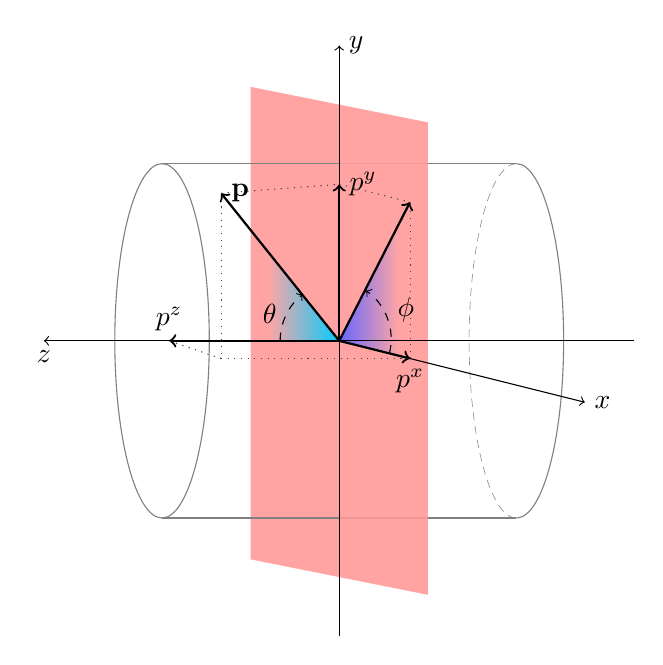
\begin{tikzpicture}[scale=0.75]
	
		\draw[gray] (-2.2,0) arc[x radius = 0.8, y radius = 3, start angle= 0, end angle= 360];
		\draw[gray] (3,3) -- (0,3); \draw[gray] (3,-3) -- (0,-3);
		\draw[gray,very thin,densely dashed] (3,3) arc[x radius = 0.8, y radius = 3, start angle= 90, end angle= 270];
		
		\draw[draw=none,fill=red!40!white,opacity=.9] (-1.5,4.3)--(1.5,3.7)--(1.5,-4.3)--(-1.5,-3.7)--cycle;

		\draw[gray] (3,-3) arc[x radius = 0.8, y radius = 3, start angle= -90, end angle= 90];
  	 	
  	 	\draw[gray] (0,3) -- (-3,3); \draw[gray] (0,-3) -- (-3,-3);
  	 	
  	 	
  	 	\draw[draw=none,  left color= blue!60!white, right color=red!35!white] (0,0)--(1,-0.25) -- (1,1.95) --cycle;
  	 	\draw[draw=none, right color= cyan!80!blue, left color=red!35!white] (0,0)--(-1.2,0) -- ( -1.2,1.53) --cycle;
  	 	\draw[->,dashed] (-1,0) arc [radius=1, start angle=180, end angle= 128] node[left =12pt, below]{$\theta$};
  	 	\draw[->,dashed] (0.85,-0.2125) arc [radius=1, start angle=-14.04, end angle= 55.3] node[below=7pt, right=8pt]{$\phi$};
  	 	
  	 	\draw[->,thick] (0,0)--(-2,2.5) node [right] {$\textbf{p}$};
  	 	\draw[->,thick] (0,0)--(1.2,2.35) node [right] {\textbf{\pt}};
  	 	\draw[->,thick] (0,0)--(-2.88,0) node [above ] {$p^{z}$};
  	 	\draw[->,thick] (0,0)--(1.2,-0.3) node [below ] {$p^{x}$};
  	 	\draw[->,thick] (0,0)--(0,2.65) node [right ] {$p^{y}$};
  	 	
  	 	\draw[thin,dotted,darkgray] (-2,2.5)--(-2,-0.3);
		\draw[thin,dotted,darkgray] (-2,-0.3)--(1.2,-0.3);
		\draw[thin,dotted,darkgray] (1.2,-0.3)--(1.2,2.35);
		\draw[thin,dotted,darkgray] (-2,2.5)--(0,2.65);
		\draw[thin,dotted,darkgray] (0,2.65)--(1.2,2.35);
		\draw[thin,dotted,darkgray] (-2,-0.3)--(-2.88,0);
		

		%===ASSI===
		\draw [->,thin] (5,0)--(-5,0) node[below]{$z$};
		\draw [->,thin] (0,0)--(4.16,-1.04) node[right]{$x$};
		\draw [->,thin] (0,-5)--(0,5) node[right]{$y$};
	
	\end{tikzpicture}
	\caption{Sketch of the reference frame used in the ATLAS detector which is represented as a simple cilinder. The $z$ axis points along the beam, the $x$ axis points toward the center of LHC ring and the $y$ axis points upwars. The polar angle $\theta$ and the azimuthal angle $\phi$ are represented. The vector $\textbf{p}$ is decomposed in its component $(p^x,p^y,p^z)$ and its transverse part $\textbf{\pt}=p^x \textbf{e}_x+p^y \textbf{e}_y$ lying in the red transverse plane in the middle is pointed out.}
\label{fig:coordinate}
\end{figure}
\begin{figure}
  \centering 
  
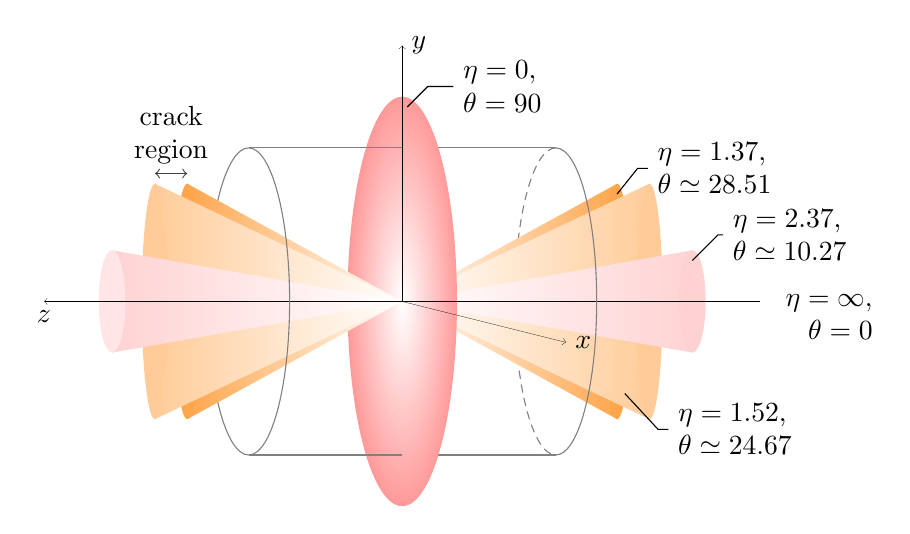
\begin{tikzpicture}[scale=0.65]
	\draw[gray,densely dashed] (3,3) arc[x radius = 0.8, y radius = 3, start angle= 90, end angle= 270];
	\draw[gray] (-3,3) arc[x radius = 0.8, y radius = 3, start angle= 90, end angle= 270];
	\draw[gray] (3,3) -- (0,3); \draw[gray] (3,-3) -- (0,-3);
	
	%eta1.37
	\draw[right color=orange!70!white, left color=white,draw=none] (0,0)--(4.2,2.3)--(4.2,-2.3) --cycle;
	\draw[fill=orange!70!white,draw=none] (4.2,2.3)arc[x radius = 0.26, y radius = 2.3, start angle= 90, end angle= 450];
	\draw[thin] (4.2,2.1) -- (4.6,2.6) -- (4.8,2.6) node[right,align=left] {$\eta=1.37$, \\$ \theta\simeq\ang{28.51}$};

	%eta1.52
	\draw[right color=orange!40!white, left color=white,draw=none] (0,0)--(4.83,2.3)--(4.83,-2.3) --cycle;
	\draw[fill=orange!40!white,draw=none] (4.83,2.3)arc[x radius = 0.26, y radius = 2.3, start angle= 90, end angle= 450];
	\draw[thin] (4.35,-1.8) -- (5,-2.5) -- (5.2,-2.5) node[right,align=left] {$\eta=1.52$, \\$ \theta\simeq\ang{24.67}$};
	
	%eta2.37
	\draw[right color=pink!70!white, left color=white,draw=none] (0,0)--(5.67,1)--(5.67,-1) --cycle;
	\draw[fill=pink!70!white,draw=none] (5.67,1)arc[x radius = 0.26, y radius = 1, start angle= 90, end angle= 450];
	\draw[thin] (5.67,0.8) -- (6.17,1.3) -- (6.27,1.3) node[right,align=left] {$\eta=2.37$, \\$ \theta\simeq\ang{10.27}$};
	
	%eta0
	\draw[inner color =white, outer color=red!40!white,draw=none] (0,0) ellipse (1.07 and 4);	
	\draw[thin] (0.1,3.8) -- (0.5,4.2) -- (1,4.2) node[right,align=left] {$\eta=0,$ \\$ \theta=\ang{90}$};
	
	%eta1.37left
	\draw[left color=orange!70!white, right color=white,draw=none] (0,0)--(-4.2,2.3)--(-4.2,-2.3) --cycle;
	\draw[fill=orange!70!white,draw=none] (-4.2,2.3)arc[x radius = 0.26, y radius = 2.3, start angle= 90, end angle= 450];
	
	%eta1.52left
	\draw[left color=orange!40!white, right color=white,draw=none] (0,0)--(-4.83,2.3)--(-4.83,-2.3) --cycle;
	\draw[fill=orange!40!white,draw=none] (-4.83,2.3)arc[x radius = 0.26, y radius = 2.3, start angle= 90, end angle= 450];
	
	%eta2.37left
	\draw[left color=pink!70!white, right color=white,draw=none] (0,0)--(-5.67,1)--(-5.67,-1) --cycle;
	\draw[fill=pink!40!white,draw=none] (-5.67,1)arc[x radius = 0.26, y radius = 1, start angle= 90, end angle= 450];
	
	\draw[<->,darkgray] (-4.83,2.5)--(-4.2,2.5);
	\draw[] node at (-4.515,2.5) [above,align=center]{crack\\ region};
	\draw[] node at (7.3,-0.3) [right,align=right]{$\eta=\infty,$\\ $\theta=\ang{0}$};

  	\draw [->,ultra thin] (7,0)--(-7,0) node[below]{$z$};
	\draw [->,ultra thin] (0,0)--(3.2,-0.8) node[right]{$x$};
	\draw [->,ultra thin] (0,0)--(0,5) node[right]{$y$};
	\draw[gray] (-3,3) arc[x radius = 0.8, y radius = 3, start angle= 90, end angle= -90];
	\draw[gray] (0,3) -- (-3,3); \draw[gray] (0,-3) -- (-3,-3);
	
	\draw[gray] (3,-3) arc[x radius = 0.8, y radius = 3, start angle= -90, end angle= 90];

\end{tikzpicture}
\caption{Notable value of $\eta$ for the corresponding $\theta$. The crack region  for\etaRange{1.37}{1.52}, along with the limit of electromagnetic calorimeter for $\eta = 2.37$, in which photons are identified, are highlighted. The gray cilinder is a sketch of the ATLAS detector. Due to left-right simmetry, the $\theta$ angle displayed represent both the value shown and their $\pi-\theta$ symmetric.}
\label{fig:pseudorapidita}
 \end{figure}

\subsection{General overview}
ATLAS geometry is mostly driven by three superconducting toroids (one barrel and two end caps). So ATLAS shows a forward/backward symmetry wrt the interaction point and a cilyndrical symmetry around the beam axis. There is also a thin superconducting solenoid surrounding the inner detector (ID), and provides a magnetic fields of about \SI{2}{\tesla}.

The ATLAS detector can be divided into three subdetectors, each one providing a precise task and accomplishing a certain measurement for a specific class of particles. The various part of ATLAS, which will be explained in this section in greater detail, and how particles behave with them is shown in \Fig{\ref{fig:behaviour}}, their coverage in pseudorapidity is given in \Tab{\ref{tab:eta}}.
\begin{description}
\item[Inner Detector] Immersed in the solenoid magnetic field, it provides charged particles momentum measurements and primary and secondary vertices measurements. It is composed of semiconductor pixel, including the Insertable B-layer which was added before the start of \RunTwo, strip detectors in its inner part and straw-tube tracking detectors with the capability to generate and detect transition radiation in its outer part. It will be described in detail in \Sect{\ref{sec:ID}}.
\item[Calorimetry system] It is composed by two kind of calorimeters: a Liquid Argon (LAr) electromagnetic calorimeter and a hadronic calorimeter. They exhibit an excellent energy and position resolution for electrons, photos and jets of hadrons, It covers a very wide range in pseudorapidity for \AetaRange{4.9}. For more detail see \Sect{\ref{sec:calo}}.
\item[Muon spectrometer] The muon spectrometer surrounds the calorimeters. It provides muon momentum measurement which is achieved with three layers of high precision tracking chambers. It includes an air-core toroid system with a long barrel and two side end-caps, which bend muon trajectory. It is described in \Sect{\ref{sec:muons}}.

\begin{figure}[pt]
\centering
\small
\fontfamily{pag}\selectfont
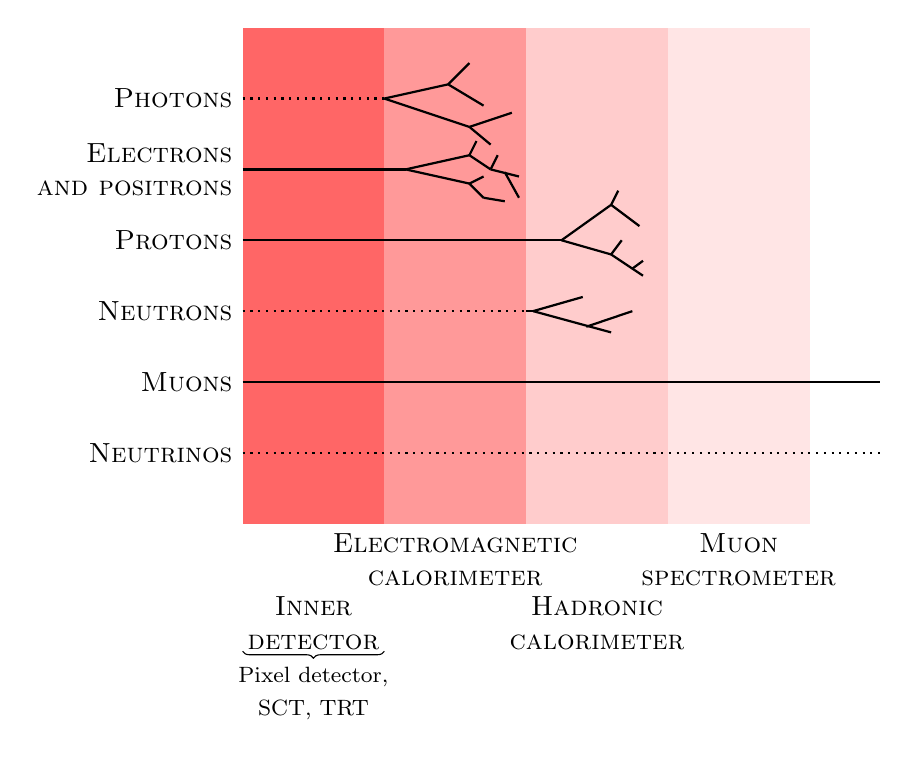
\begin{tikzpicture}[scale=0.9]
	\draw[draw=none,fill=red!60!white] (0,0) rectangle +(2,7);
	\draw[draw=none,fill=red!40!white] (2,0) rectangle +(2,7);
	\draw[draw=none,fill=red!20!white] (4,0) rectangle +(2,7);
	\draw[draw=none,fill=red!10!white] (6,0) rectangle +(2,7);
	
	\draw[thick,dotted] node[left] at (0,6) {\scshape Photons};
		\draw[dotted,thick] (0,6)--(2,6);
		\draw[thick] (2,6)--(2.9,6.2);
			\draw[thick] (2.9,6.2)--(3.2,6.5);
			\draw[thick] (2.9,6.2)--(3.4,5.9);
		\draw[thick] (2,6)--(3.2,5.6);
			\draw[thick] (3.2,5.6)--(3.5,5.35);
			\draw[thick] (3.2,5.6)--(3.8,5.8);
	\draw[thick,dotted] node[left,align=right] at (0,5) {\textsc {Electrons}\\ \textsc{and positrons}} ;
		\draw[thick] (0,5)--(2.3,5);
			\draw[thick] (2.3,5)--(3.2,5.2);
				\draw[thick] (3.2,5.2)--(3.3,5.4);
				\draw[thick] (3.2,5.2)--(3.5,5);
					\draw[thick](3.5,5)--(3.6,5.2);
					\draw[thick](3.5,5)--(3.9,4.9);
						\draw[thick](3.7,4.96)--(3.9,4.6);
			\draw[thick] (2.3,5)--(3.2,4.8);
				\draw[thick] (3.2,4.8) --(3.4,4.9);
				\draw[thick] (3.2,4.8) --(3.4,4.6);
					\draw[thick] (3.4,4.6) -- (3.7,4.55);
	
	\draw[thick,dotted] node[left,align=right] at (0,4) {\textsc{Protons}};
		\draw[thick] (0,4)--(4.5,4);
			\draw[thick] (4.5,4) -- (5.2,4.5);
				\draw[thick] (5.2,4.5)--(5.3,4.7);
				\draw[thick] (5.2,4.5)--(5.6,4.2);
			\draw[thick] (4.5,4) -- (5.2,3.8);
				\draw[thick] (5.2,3.8) -- (5.35,4);
				\draw[thick] (5.2,3.8) -- (5.5,3.6);
					\draw[thick] (5.5,3.6) -- (5.65,3.71);
					\draw[thick] (5.5,3.6) -- (5.65,3.5);
	\draw[thick,dashed] node[left] at (0,3) {\scshape Neutrons};
		\draw[thick,dotted] (0,3)--(4,3);
		\draw[thick] (4,3)--(4.1,3);
			\draw[thick] (4.1,3)--(4.8,3.2);
			\draw[thick] (4.1,3)--(5.2,2.7);
				\draw[thick] (4.85,2.78)--(5.5,3);
	
	\draw[thick] node[left] at (0,2) {\scshape Muons} (0,2) -- (9,2);	
	\draw[thick,dotted] node[left] at (0,1) {\scshape Neutrinos} (0,1) -- (9,1);
	
	\node[align=center] at (1,-1.4) {\scshape Inner\\ \scshape detector};
	\node[align=center] at (3,-.5) {\scshape Electromagnetic\\ \scshape calorimeter};
	\node[align=center] at (5,-1.4) {\scshape Hadronic\\ \scshape calorimeter};
	\node[align=center] at (7,-.5) {\scshape Muon\\ \scshape spectrometer};
	\draw [decorate,decoration={brace}] (2,-1.8)--(0,-1.8);
	\node[align=center] at (1,-2.4) {\footnotesize Pixel detector,\\ \footnotesize SCT, TRT};
\end{tikzpicture}
\caption{Particle behavior inside the various parts of the ATLAS detector, dotted lines are invisible to the various detectors. }
\label{fig:behaviour}
\end{figure}

\begin{table}[tp]
	\centering
	\begin{tabular}{lc}
	\toprule
	Detector & Pseudorapidity range\\
	\midrule
	Inner detector& \AetaRange{2.5}\\
	EM calorimeter barrel& \AetaRange{1.475}\\
	EM calorimeter end-cap, outer weel& \etaRange{1.375}{2.5}\\
	EM calorimeter end-cap, inner weel& \etaRange{2.5}{3.2}\\
	Hadronic tile calorimeter barrel& \AetaRange{1.0}\\
	Hadronic tile calorimeter extended barrel& \etaRange{0.8}{1.7}\\
	Hadronic end-cap calorimeter (HEC)& \etaRange{1.5}{3.2}\\
	Hadronic Forward calorimeter (FCAL)& \etaRange{3.1}{4.9}\\
	Muon spectrometer& \AetaRange{2.7}\\
	\bottomrule
	\end{tabular}
	\caption{Table listing the pseudorapidity range for every part of the ATLAS detector}
	\label{tab:eta}

\end{table}

\end{description}

\subsection{Inner Detector}
\label{sec:ID}
\begin{figure}[tp]
\centering
\includegraphics[width=0.8\textwidth]{LHC_ATLAS/ID}
\caption{Cut-away view of the ATLAS inner detector.}
\label{fig:id}
\end{figure}

The Inner Detector (ID), \Fig{\ref{fig:id}}, is a tracking detector and it is designed to provide precise tracks reconstruction, excellent momentum resolution and both primary and secondary vertices measurements. For the purpose of tracking, great precision measurement must be performed so that an high granularity is strongly required. Indeed every \SI{25}{\ns} about \num{1000} particles emerge from the interaction point within a $\eta$ cone of \num{2.5}. Tracking charged particles is very crucial to help other detectors to distinguish between two similar particles. Showers left in the electromagnetic calorimeter by electron and photons are very similar, the only way we have to decide which particle has passed in the detected is looking whether tracks were left in the front of the calorimeter.

\begin{figure}[pt]
\centering
\includegraphics[width=0.8\textwidth]{LHC_ATLAS/IDCrossSection}
\caption{Cross section of the inner detector.}
\label{fig:xsecID}
\end{figure}

The ID is contained within a cylindrical region of radius \SI{1.05}{\m} and lenght \SI{6.2}{\m}. It is immersed in a \SI{2}{\tesla} solenoidal magnetic field and it consists of three independent and complementary parts, as pictured in \Fig{\ref{fig:xsecID}}, which are the Pixel Detector, SemiConductor Tracker (SCT) and the Transition Radiation Tracker (TRT).

The Pixel Detector, covering the \AetaRange{2.5} range, is the closest detector to the beam reaching about \SI{33.25}{\mm} in distance with the Insertable B-layer (IBL) added during LS1. In the barrel region, pixel sensors are arranged on three concentric cylinders around the beam axis while in the end-cap regions they are organized in disks perpendicular to the beam axis. A Pixel sensor is a \si{16.4} $\times$ \SI{60.8}{\mm} wafer of silicon with \num{46080} pixels with a size in $R$-$\phi \times z$ of  \si{50} $\times$ \SI{400}{\um\squared} each. Thanks to its triple layer, the detector provides three measurement points to reconstruct the track with a resolution of \SI{10}{\um} in the direction orthogonal to its disposition and \SI{115}{\um} in the longitudinal one. The pixel detector has approximately \num{92} million readout channels overall.

The SCT is devoted to reconstruct particles momenta. It covers a $R$ distance between \SI{299}{\mm} and \SI{514}{\mm}  from the beam pipe and it consists of modules of silicon strips arranged in four concentric barrels and two end-caps of nine disks each. In the barrel it uses small angle stereo strips to measure a particle's coordinate, with a particular set parallel to the beam axis for measuring $R$ and $\phi$, while in the end-cap it uses a set of strips running radially. 
{\bfseries To get a measure of the $z$ coordinate in the barrel a set of stereo strips at an angle of \SI{40}{mrad} overlaps the one underneath which is kept parallel to the $z$ axis.}
Here eight strip layers corresponding to four space points are crossed by each track. The total number of readout channels in the SCT is approximately 6.3 million, each of them providing a precision of \SI{17}{\um} in the $R$-$\phi$ plane and \SI{180}{\um} in $z$ direction for barrel and in $R$ direction for the end-cap region.

The outer part of the ID is a TRT which occupies a cilinder of radii \SI{554}{\mm} and \SI{1082}{\mm}. The detecting elements are drift tubes (straws) with a diameter of \SI{4}{mm} and \SI{144}{cm} long in the barrel region, where they are parallel to the beam axis being cut in a half at $\eta =0$, and \SI{37}{\cm} long in the end-cap region where they are distributed radially. It provides information only on $R$-$\phi$ coordinates with a resolution of  only \SI{200}{\um} per straw, much less than the other two detectors. On the other hand it provides a very large number of hits per track, which is about \num{36}. The TRT has about \num{298000} straws in total. {\bfseries Its tecnology is based on transition radiation which occurs whenever a charged particle crosses two media with different refractive index. Tracks left, for instance, by electrons and charged pions is very similar. In order to distinguish them one can build this system so that a radiation is emitted only when an electron crosses a straw.}

The combination of precision trackers in the innermost shell with the TRT at a larger radius gives very robust pattern recognition and high precision measurements. For instance the TRT's straws hit at large radius contributes significantly to determine a particle's momentum by compensating their small precision with longer measured track and larger number of hits.

Finally the ID typical momentum resolution is $\frac{\sigma_{\pt}}{\pt}=0.05\%\pt\oplus1\%$.

The Inner Detector system provides tracking measurements in a range matched by the precision measurements of the electromagnetic calorimeter which will be described in the next section.

\subsection{Calorimetry}
\label{sec:calo}
Calorimeters are the detectors dedicated to energy measurements for both neutral an chrged particles, except for muons. To improve the precision of the missing transverse momentum (\met) the pseudorapidity range extends up tp $\eta=4.9$, with a full $\phi$ coverage. Nevertheless there is a blind zone in \etaRange{1.37}{1.52} called \emph{crack region} where the barrel/end-cap transition happens.

In ATLAS the calorimetry system, represented in \Fig{\ref{fig:Calos}}, is composed by two subsystems: the electromagnetic (EM) calorimeter, optimized to measure photons and electrons thanks to its finer granularity, and the hadronic calorimeter which measure the energy and position of jets of hadrons. Both of them are sampling calorimeters, which means they are made of a series of active and absorber material samples.

An important feature in building them is the calorimeter depth. They must provide good containment for electromagnetic and hadronic showers limiting the amount of electrons, photons and hadrons leaking into the muon spectrometer.

\begin{figure}[tp]
\centering
\includegraphics[width=0.8\textwidth]{LHC_ATLAS/Calorimetry}
\caption{Cut-away view of ATLAS calorimetry system. It develops around the inner detector in gray and it is composed by the electromagnetic and hadronic calorimers.}
\label{fig:Calos}
\end{figure}

\subsubsection{Electromagnetic Calorimeter}
\begin{figure}[tp]
\centering
\includegraphics[width=0.55\textwidth]{LHC_ATLAS/EMcalo}
\caption{Schematic view of a fraction of the EM calorimeter showing its accordion geometry and pointing out the segmentation in ``strips'', ``middle'' and ``back'', along with their granularity, in the  barrel region.}
\label{fig:EMlayers}
\end{figure}

The EM calorimeter is designed to detect, measure and track electrons and photons and it is part of the LAr calorimetry. Indeed it adopts entirely this tecnology consisting in a Liquid Argon ionization chamber using lead as absorber. It is composed by two half-barrels, separated at $\eta=0$ by a \SI{4}{\mm} gap, covering \AetaRange{1.475}. Two end-caps (EMEC), composed by a outer and an inner weel, cover the range in pseudorapidity respectively to \etaRange{1.375}{2.5} and \etaRange{2.5}{3.2} each housed in its own cryostat. Precision measurements, however, are performed up to $\eta=2.37$ where the strips in the ID ends;

It is built following an accordion geometry which naturally guarantee a full $\phi$ coverage without any cracks. In the barrel the accordion waves are parallel to the beam axis, running in $\phi$, and their folding angle varies with $R$ keeping the LAr gaps pretty constant. In the endcaps, the waves run axially and the folding angle varies with radius.

In the longitudinal direction and for \AetaRange{2.5}, where precise measurements take place, the EM barrel calorimeter is segmented into three longitudinal sections while the inner wheel, for $\abs\eta>2.5$, in two sections. In barrel the three sections are called ``strips'', ``middle'' and ``back'' as shown in \Fig{\ref{fig:EMlayers}}. The strips layer has the highest granularity which reaches \mbox{$0.008 \times 0.1 \left(\Delta \eta \times \Delta \phi \right)$}, needed to distinguish between a decayed \pizero from a real photon. The middle calorimeter layer collects the largest fraction of the energy of eth electromagnetic showers and the back detects their tails and prevents the shower to reach the outer hadronic calorimeter. The total thickness of the EM calorimeter is greater than 22 radiation lengths ($X_0$), which is defined as the mean distance over which a high energy electron loses $1/e$ of its energy by bremsstrahlung, in the barrel and greater than 24 $X_0$ in the end-caps.
  
Going through the ID, energy loss for photons and electrons might happen and it must be taken into account. A presampler, which is a very thin Liquid-Argon layer ($\sim \SI{11}{\mm}$), is added before the calorimeter to recover this kind of energy loss.

\subsubsection{Hadronic Calorimeter}
The Hadronic Calorimeter is characterized by three parts: the tile calorimeter in the barrel region for \AetaRange{1.7}, the LAr hadronic forward (FCal) in the \etaRange{1.4}{3.2} region, and end-cap (HEC) calorimeter for \etaRange{3.2}{4.9}. 

The Tile Calorimeter, placed just outside the EM calorimeter in the radial direction, is a sampling calorimeter which uses steel as absorber and a scintillator as an active medium. It can be divided in the proper barrel region and two extended barrels, both extending from an inner radius of \SI{2.28}{\m} to an outer one of \SI{4.25}{\m} and segmented in depth in three layers. The barrel covers the region \AetaRange{1.0} and the two extended barrels extend the covering to $\eta=1.7$. While speaking of hadrons, the interaction lenghts ($\lambda$), i.e. the mean distance between two hadron-nuclear matter interaction, is used instead of radiation lenght to define the depth of the calorimeter. The interaction lenght can be computed as $\lambda \simeq \frac{A^{1/3}}{\rho}$ where $A$ is the mass number for a specific atom and $\rho$ is the nuclear density. The total detector thickness in the tile-instrumented region is \SI{9.7}{\lambda} at $\eta = 0$ and \SI{10}{\lambda} in the extended barrel.

The HEC and FCal parts use the same technology as in the EM calorimeter so that their active medium is Liquid Argon but their absorber can be tungsten or copper. The HEC is located directly behind the EM end-cap calorimeter, sharing the same cryostat, and it consists of two independent wheels per end-cap. Each weel is divided into two segments in depth, for a total of four layers per end-cap. The FCal completes the $\eta$ coverage of the calorimeter system being located in \etaRange{3.2}{4.9}. It consists of three modules in each end-cap: the first, made of copper, is suited for electromagnetic measurements, while the other two, made of tungsten, measure the energy of hadronic interactions.

\subsection{Muon Spectrometer}
\label{sec:muons}
The Muon Spectrometer is the outermost detector in ATLAS which is shown in \Fig{\ref{fig:muons}}. Its functioning is based on the magnetic deflection of muons in the large superconducting air-core toroid magnets built in such a way the magnetic field is almost orthogonal to muons path. For \AetaRange{1.4} bending is achieved thanks to the barrel toroids, for \etaRange{1.6}{2.7} muons are bent by two smaller end-cap toroids and in the intermediate, or transition region (\etaRange{1.4}{1.6}) the deflection occurs from a combination of the two fields. Bending power is computed by the field integral $\int B_{\bot}\,dl$ where $B_{\bot}$ is the field perpendicular to the muons trajectory and the integral is evaluated along the infinitesimal path covered by muons inside the spectrometer. The barrel toroid provides \SI{1.5}{\tesla \metre} to \SI{5.5}{\tesla \metre} and the end-cap toroid gives from \SI{1}{\tesla \metre} to \SI{7.5}{\tesla \metre}. The magnetic field is continuously monitored by almost 1800 Hall sensors distributed throughout the spectrometer: this is crucial in order to calculate the bending power along the muon trajectory to a few parts in a thousand.

In the barrel region, tracks are measured in chambers arranged in three cylindrical layers around the beam axis while in transition and end-cap region three-layered chambers are located in planes orthogonal to the $z$-axis. The tracking chamber are made of Monitored Drift Tube (MDT) which pursue high-precision tracking along almost the whole $\eta$ range. They are made of cylindrical aluminum drift tube being filled with gas which gets ionized when a muon passes by. Charge is collected by a wire held at high potential. Cathode-strip chambers (CSC) covers \etaRange{2}{2.7}. They are multiwire proportional chambers with cathodes segmented into strips with an higher rate capability and high granularity.     

The muon spectrometer has its own trigger system which extends over \AetaRange{2.4} and uses Resistive Plate Chambers (RPC) and Thin-gap Chambers (TGC) in barrel and end-cap regions respectively.{\bfseries Its typical momentum resolution $\frac{\sigma_{\pt}}{\pt}$ varies from 2\% to 5\% in the range between \SI{1}{\TeV} and \SI{10}{\TeV}.}

\begin{figure}[pt]
\centering
\includegraphics[width=0.7\textwidth]{LHC_ATLAS/Muons}
\caption{Cut-away view of the ATLAS muon system.}
\label{fig:muons}
\end{figure}

\subsection{Forward Detectors}
Three smaller detector systems cover the ATLAS forward region. LUCID (LUminosity measurement using Cerenkov Integrating Detector) at \SI{\pm 17}{\m}, along the beam, and ALFA (Absolute Luminosity For ATLAS) located at \SI{\pm 240}{\m} are used to measure the istantaneous luminosity delivered to ATLAS. The third system is the Zero-Degree Calorimeter (ZDC), located at \SI{\pm 140}{\m}, which is used in determining the centrality of heavy-ion collisions.

\subsection{Trigger system}
The rate of events expected rate at the LHC designed luminosity is \SI{1}{\GHz}, as mentioned in the previous Section, on the other hand the maximum event rate that ATLAS can record is \SI{\sim 1000}{\Hz}. It is evident that an appropriate trigger system must be used so that only events that could have potential physical interest would be recorded. There are two distinct levels of trigger: L1 and the High Level Trigger (HLT), which sums up the previous L2 and Event Filter. Each trigger level refines the decisions made at the previous level using more refined quantities at each step, and, where necessary, applies additional selection criteria.

L1 looks for high-\pt particles such as electrons, photons, $\tau$-leptons decaying into hadrons as well as large \met and defines one or more Region-of-Interest (RoI) which is a $\Delta \eta \times \Delta \phi$ region in which interesting events can be found. It uses information coming from a subset of detectors which are processed by the central trigger processor. The operating time is about \SI{2.5}{\um} which reduces the event rate down to \SI{100}{\kHz}.

The final stage of the selection is made by the Event Filter (EF) which reduces the rate to a reasonable \SI{1}{\kHz}. It selects events using the full granularity avaliable for each subdetector, and store them as raw data (RDO) for offline analysis. Every event is computed in about \SI{4}{\s}. Performance of L1 and High Level Trigger are show respectively in \Fig{\ref{fig:L1}} and \Fig{\ref{fig:HLT}}.

\begin{figure}[t]
\centering
\subfloat[][L1 performance]
{\includegraphics[width=.55\textwidth]{LHC_ATLAS/Time_L1GroupRate_Stack_2016_07} \label{fig:L1}} \\

\subfloat[][HLT performance]
{\includegraphics[width=.55\textwidth]{LHC_ATLAS/Time_HLTGroupRate_Stack_2016_07} \label{fig:HLT}}

\caption{Physics trigger group rates at the High Level Trigger (HLT) and the first trigger level (L1) as a function of the number of luminosity blocks which correspond to on average \SI{60}{\s} per luminosity block in a fill taken in July 2016 with a peak luminosity of L = \SI{1.02 e34}{\per\cm\squared\per\s}. We can notice the sawthoot behavior given by loosing of trigger requirements while the beam gets less perfect.}
\end{figure}





